\chapter{Programm Launch}
In diesem Kapitel wird beschrieben, wie das kompilierte uForth Programm aus der IDE gestartet werden kann und was dafür implementiert wurde.

\section{Launch}

Im Eclipse werden zwischen zwei Launch Möglichkeiten unterschieden. Der unterschied zwischen beiden wird in den nächsten Kapiteln erklärt.

\begin{figure}[H]
	\centering
		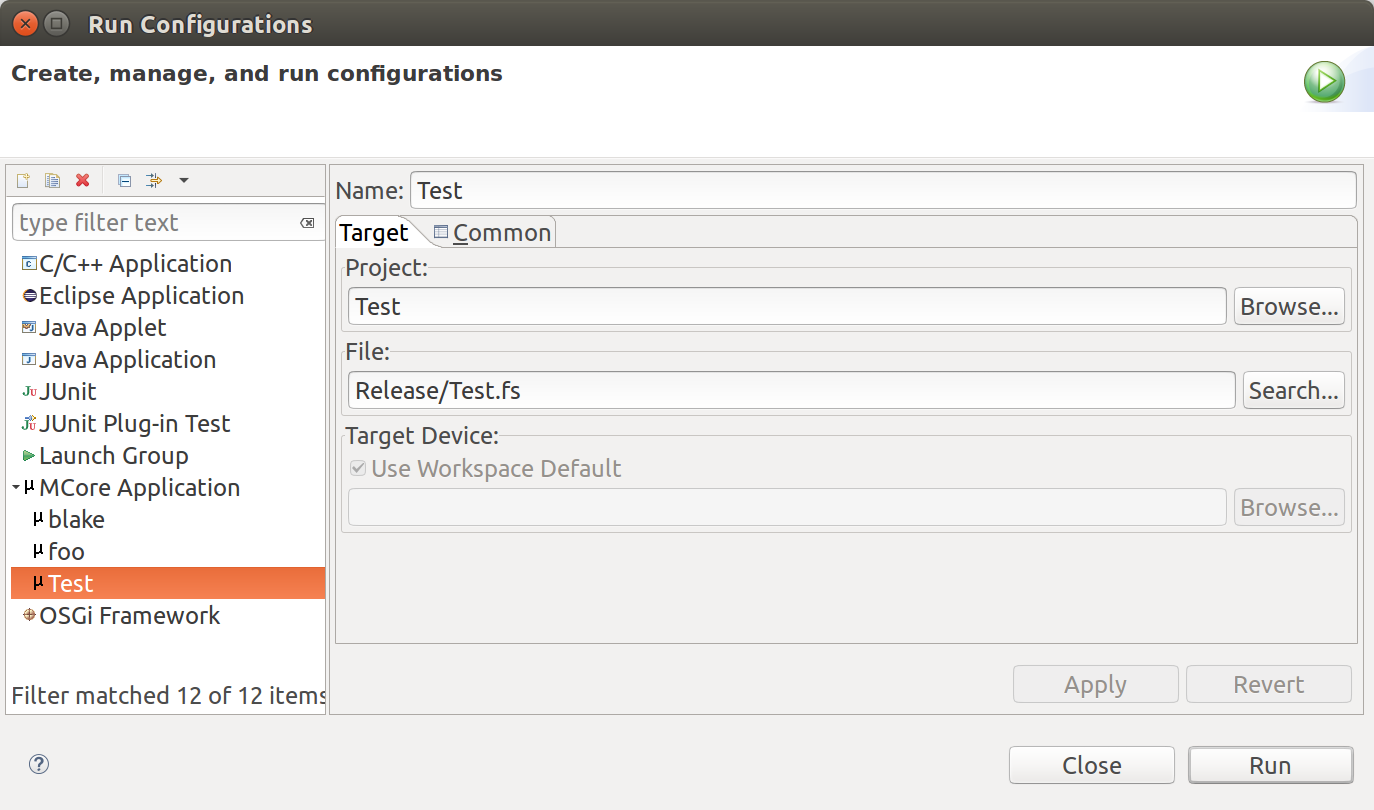
\includegraphics[scale=0.3]{launch/run.png}
		\caption{Der Launch Configuration Dialog. Im Dialog kann eine neue MCore Launch Konfiguration erstellt werden. Um eine gültige Konfiguration zu erstellen muss das Projekt und das Forth File, welches gestartet werden soll angegeben werden.}
		\captionsetup{margin=0cm,font={footnotesize}}
		\label{fig:extensionpoint}
\end{figure}

\newpage
\subsection{Run}

Mit der Run Konfiguration wird zuerst der Loader in den Forth Workspace kopiert (dieser muss in einer Umgebungsvariable definiert sein). Danach wird der Forth Prozess gestartet und der Umbilical Port mittels \verb!Umbilical: /dev/ttyUSBX! gesetzt. Der Umbilical Port und der Loader müssen in der MCore Settings Page gesetzt werden (Siehe Kapitel \ref{settingschapter}). Falls der Umbilical Port ungültig ist, wird beim starten des Programmes eine Fehlermeldung gezeigt.

\begin{figure}[H]
	\centering
		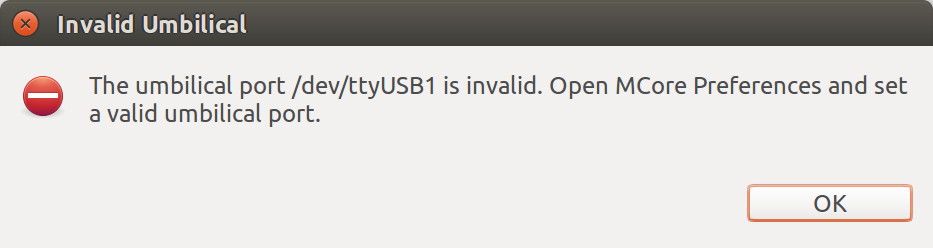
\includegraphics[scale=0.4]{launch/invalidumbilical.png}
		\caption{Dialog, welcher angezeigt wird, wenn ein Program gestartet wird und der Umbilical Port nicht gültig ist. Der Port kann in der MCore Preference Page geändert werden.}
		\captionsetup{margin=0cm,font={footnotesize}}
		\label{fig:extensionpoint}
\end{figure}

\subsection{Debug}

In der Debug Konfiguration werden zusätzlich noch alle Funktionen des gestarteten Forth Files disassembled. Dies wird gemacht, dass der Debugger die Funktionen in einem File anzeigen kann. Es kann nicht der vom Compiler generierte Code genommen werden, da der Forth Cross-Compiler noch Optimierungen am Code vornimmt, deshalb müssen die Funktionen zur Laufzeit noch disassemnbled werden.

